\section*{Derivace funkce}

Derivace funkce v bodě umožňuje popsat, jak rychle se funkce v takovém bodě funkce mění.

\subsection*{Lineární funkce}

Lineární funkce jsou funkce tvaru $y(x) = ax+b$, kde $a$ a $b$ jsou určité koeficienty. Víme, že grafem lineární funkce je přímka a také, jaký vliv na ni mají $a$ a $b$:
\begin{itemize}
    \item Koeficient $b$ je tzv. \textbf{absolutní koeficient}. Udává hodnotu funkce v bodě nula. Čím je $b$ větší, tím více posouvá graf funkce $y(x)$ nahoru.
    \item Koeficient $a$ je tzv. \textbf{lineární koeficient} neboli \textbf{směrnice} přímky. Udává sklon přímky. Čím je $a$ větší, tím je graf funkce strmější. Pro $a>0$ je funkce rostoucí, pro $a=0$ přejde funkce na obyčejnou konsatntní funkci $y=b$ s nulovým sklonem, pro $a<0$ je funkce klesající.
\end{itemize}

Uvažujme nyní lineární funkce $y(x)=ax+b$ a nějaký pevný bod $x_0$ s funkční hodnotou $y(x_0)$. Ptejme se nyní, co se stane, zvětšíme-li hodnotu $x$ o nějakou vzdálenost $\D x$. Jak se změní funkční hodnota? Nakreslíme-li si situaci, vidíme, že se hodnota změní o $\D y = \D x \cdot a$. Můžeme tedy zapsat
\begin{align}
    a = \frac{\D y}{\D x} \:.
\end{align}
Představme si třeba funkci $y(x)=2x+4$ a bod $x_0=2$. Posuneme-li se o $\D x = 1$, pak se změní hodnota $y$ o $\D y = a \cdot \D x = 2 \cdot 1 = 2$. Posuneme-li se o $\D x = 2$, změní se hodnota $y$ o $\D y = 2 \cdot 2 = 4$, atd\dots

\begin{figure}[H]
    \centering
    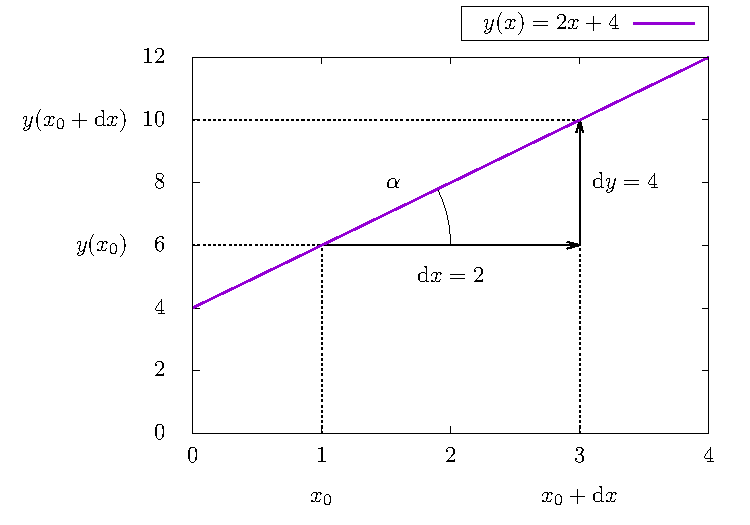
\includegraphics{Gnuplot/cv8/Figures/primka-graf.pdf}
    \caption{Znázorněna funkce $y(x)=2x+4$. Zafixujme bod $x_0=2$ s hodnotou $y(x_0)=6$. Pokud se změní $x$ o hodnotu $\D x = 2$, změní se hodnota $y$ o $\D y = \D x \cdot 2 = 4$.}
\end{figure}

To, že při posunu o $\D x$ snadno spočteme $\D y$ pouhým vynásobení číslem, je vlastnost, která platí pouze pro lineární funkce. Proto jsou vlastně lineární funkce tak speciální. U složitějších funkcí už obecně záleží na tom, jak velké je $x$ a $\D x$. Uvažte například kvadratickou funkci, tam už přírůstek $\D y$ bude pokaždé jiný.

\subsection*{Derivace jako tečna funkce}

Pakliže však bude funkce \uv{dostatečně rozumná} a ono $\D x$ dostatečně malé, máme návod na to, jak určit malou změnu v $\D y$. Můžeme se totiž na nějakém malém okolí bodu $x_0$ pokusit aproximovat funkci její \textbf{tečnou}. Jak vytvořit tečnu ke křivce v daném bodě? Začneme tím, že vytvoříme \textbf{sečnu}, přímku spojující dva body na grafu funkce. Jeden bod bude $(x_0,f(x_0))$. Druhý bod vezměme tak, že posuneme bod $x_0$ o nějakou vzdálenost $h$ a získáme bod $(x_0+h,f(x_0+h))$.

\begin{figure}[H]
    \centering
    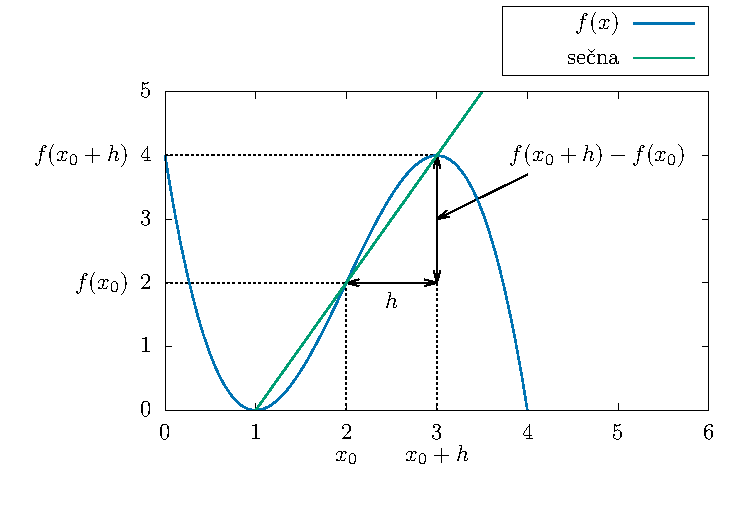
\includegraphics{Gnuplot/cv8/Figures/secna-graf.pdf}
    \caption{Příklad konstrukce sečny k nějaké funkci (modrá). Vezmeme bod $x_0=2$ s funkční hodnotou $f(x_0)=2$. Druhý bod vezmeme tak, že k $x_0$ přičteme $h=1$. Odpovídající funkční hodnota je $f(x_0+h)=4$. Takto získané body propojíme přímkou (zelená).}
\end{figure}

Nyní si všimneme, že čím blíže bude druhý bod prvnímu, tím lépe se sečna podobá tečně. Pokud budeme zmenšovat onu vzdálenost $h$ mezi dvěma body (přičemž $x_0$ ponecháváme stále na místě), bude se směrnice sečen stále více přibližovat směrnici tečny.

\begin{figure}[H]
    \centering
    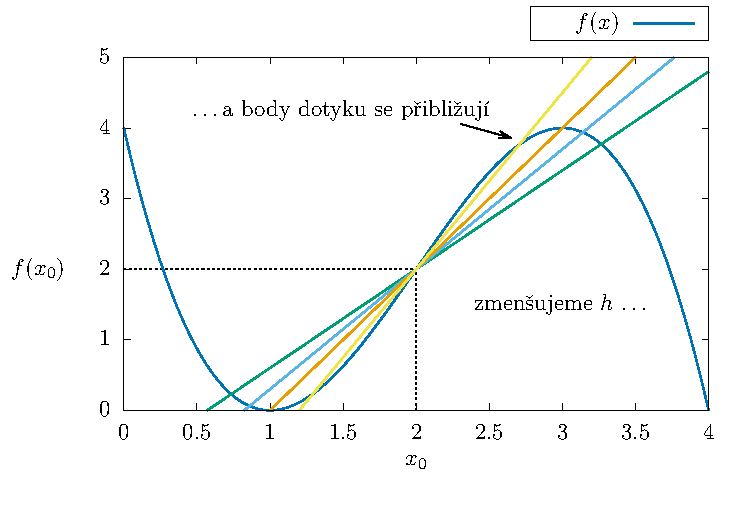
\includegraphics{Gnuplot/cv8/Figures/priblizovani-graf.pdf}
\end{figure}

Až nakonec pro $h \rightarrow 0$ přejdou sečny skutečně v tečnu.

\begin{figure}[H]
    \centering
    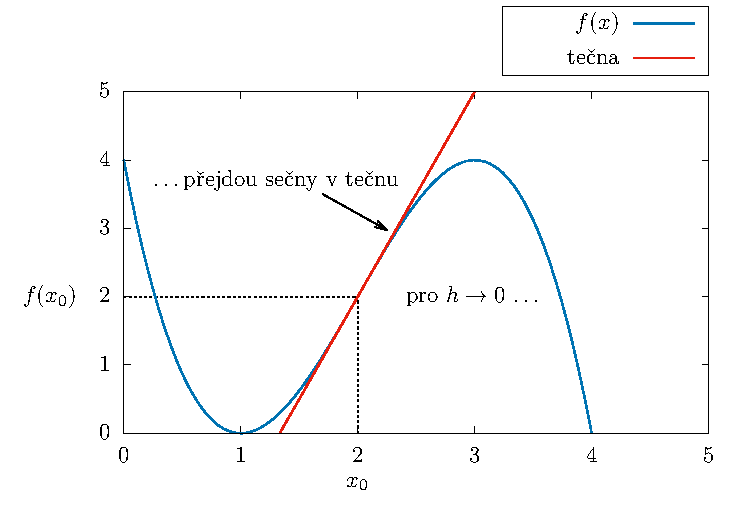
\includegraphics{Gnuplot/cv8/Figures/tecna-graf.pdf}
\end{figure}

Pokud nyní vezmeme $\D x$ dostatečně malé, nebude nám vadit, když místo skutečné hodnoty $\D y$ budeme počítat s přibližnou hodnotou, kterou nám bude dávat bod na tečně.

Vraťme se k předchozímu obrázku. Jaká je směrnice zelené sečny? Je to zase podíl toho, o kolik se změnila funkční hodnota, a toho, o kolik jsme se posunuli:
\begin{align}
    \text{směrnice sečny} = \frac{\text{o kolik se změní funkce}}{\text{o kolik se posuneme}} = \frac{f(x_0+h)-f(x_0)}{(x_0+h)-x_0} = \frac{f(x_0+h)-f(x_0)}{h} \:.
\end{align}
Směrnici tečny získáme limitním procesem
\begin{align}
    \text{směrnice tečny} = \lim_{h \rightarrow 0} \text{směrnice sečny} = \lim_{h \rightarrow 0} \frac{f(x_0+h)-f(x_0)}{h} \:.
\end{align}
Získáváme tak vztah pro \textbf{derivaci funkce $f$ v bodě} $x_0$:
\begin{align}
    \boxed{\frac{\D f}{\D x} (x_0) = f'(x_0) = \lim_{h \rightarrow 0} \frac{f(x_0+h)-f(x_0)}{h}} \:.
\end{align}
Ještě jednou, derivace funkce $f$ v bodě $x_0$ představuje směrnici tečny k takové funkci v bodě $x_0$. K čemu je to dobré? Pokud se posuneme o nějaké $\D x$ a ptáme se, o jakou hodnotu $\D f$ se funkce $f$ změní, můžeme použít jednoduchý vztah:
\begin{align}
    \D f = \D x \cdot f'(x_0) \:.
\end{align}
Dokonce si můžeme napsat celý předpis pro tečnu:
\begin{align}
    \text{rovnice tečny} = y(x) = f'(x_0) \cdot (x-x_0) + f(x_0) \:.
\end{align}
Přírůstek $x-x_0$ je právě posunutí mezi $x_0$ a $x$. Zajímá-li nás hodnota tečny v bodě $x$, stačí takové posunutí vynásobit derivací funkce $f'(x_0)$ a přičíst ještě funkční hodnotu $f(x_0)$.

\subsection*{Jak derivaci počítat?}

Můžeme ji počítat přímo z definice.

\begin{example}[Derivace lineární funkce]
    Výše jsme uvedli, že lineární funkce $y(x)=ax+b$ má všude stále stejnou směrnici $a$. To znamená, že lineární funkce splývá se svou tečnou a derivace by měla být rovna směrnici $a$. To se dá samozřejmě ukázat i matematicky:
    \begin{align}
        y'(x_0) = \lim_{h \rightarrow 0} \frac{y(x_0+h)-y(x_0)}{h} = \lim_{h \rightarrow 0} \frac{[a(x_0+h)+b]-[a x_0 + b]}{h} = 
        \lim_{h \rightarrow 0} \frac{ah}{h} = \lim_{h \rightarrow 0} a = a \:. 
    \end{align}
    Vidíme, že derivace je všude rovna $a$, nezávisle na tom, v jakém bodě $x_0$ ji počítáme.
\end{example}

\begin{example}[Kvadratická funkce]
    Jak to bude u kvadratické funkce $f(x)=x^2$? Čekáme, že zde již derivace bude záviset na bodě $x_0$, kde ji počítáme. Parabola se totiž stává stále strmější a strmější. Výpočet dává
    \begin{align}
        f'(x_0) = \lim_{h \rightarrow 0} \frac{[(x_0+h)^2]-[x_0^2]}{h} = 
        \lim_{h \rightarrow 0} \frac{2 x_0 h + a h^2 }{h} =
        \lim_{h \rightarrow 0} (2 x_0 + ah) = 2 x_0 \:.
    \end{align}
    Derivace je tedy různá v každém bodě $x_0$. Čím větší je bod $x_0$, tím větší je derivace. To přesně odpovídá tomu, že je ve vzdálenějších bodech parabola strmější a strmější.
\end{example}

\begin{example}[Nepřímá úměrnost]
    Jaká bude derivace u funkce $g(x)=\frac{1}{x}$? Čekáme, že derivace určitě záporná, neboť nepřímá úměrnost je klesající, tečna bude tedy taky klesající. Navíc čím větší bude $x_0$, tím se pokles funkce zpomaluje. Výpočtem ukážeme
    \begin{align}
        g'(x_0) = \lim_{h \rightarrow 0} \frac{\frac{1}{x_0+h}-\frac{1}{x_0}}{h} =
        \lim_{h \rightarrow 0} \frac{1}{h} \frac{(x_0)-(x_0+h)}{(x_0+h)x_0} = 
        \lim_{h \rightarrow 0} \frac{-h}{h (x_0+h) x_0} = 
        \lim_{h \rightarrow 0} \frac{-1}{(x_0+h) x_0} = -\frac{1}{x_0^2} \:.
    \end{align}
    To je přesně to, co jsme čekali.
\end{example}

Počítání z definice je ale poměrně zdlouhavé, jakmile jsou předpisy pro funkce složitější. Naštěstí platí stejná pravidla pro aritmetiku derivací, jako pro aritmetiku limit.